\documentclass{beamer}
\usepackage{listings}
\lstset{
%language=C,
frame=single, 
breaklines=true,
columns=fullflexible
}
\usepackage{subcaption}
\usepackage{url}
\usepackage{tikz}
\usepackage{tkz-euclide} % loads  TikZ and tkz-base
%\usetkzobj{all}
\usetikzlibrary{calc,math}
\usepackage{float}
\newcommand\norm[1]{\left\lVert#1\right\rVert}
\newcommand{\Lagr}{\mathcal{L}}
\renewcommand{\vec}[1]{\mathbf{#1}}
\providecommand{\pr}[1]{\ensuremath{\Pr\left(#1\right)}}
\usepackage[export]{adjustbox}
\usepackage[utf8]{inputenc}
\usepackage{amsmath}
\usetheme{Madrid}

\title{Research Paper - Presentation}
\author{Dontha Aarthi - CS20BTECH11015}

\begin{document}
\begin{frame}
\titlepage
\end{frame}
\section{Title and Authors}
\begin{frame}
\frametitle{Title and Authors}
\begin{block}{Title}
Deep Minimax Probability Machine

\end{block}
\begin{block}{Authors}
\begin{enumerate}
    \item Lirong He, SMILE Lab, School of Computer Science and Engineering
    University of Electronic Science and Technology of China Chengdu, China, lirong he@std.uestc.edu.cn
    \item Ziyi Guo, Cloud and Smart Industries Group Tencent
Guangzhou, China, ziyiguo94@gmail.com
    \item Kaizhu Huang, Department of EEE, Xi’an Jiaotong-Liverpool University, Suzhou, China, Kaizhu.Huang@xjtlu.edu.cn\\
    \item Zenglin Xu, SMILE Lab, School of Computer Science and Engineering, University of Electronic Science and Technology of China
Chengdu, China, Center for Artificial Intelligence, Peng Cheng Laboratory
Shenzhen, China, zenglin@gmail.com
\end{enumerate}

\end{block}
\end{frame}
\section{\textbf{Introduction}}
\subsection*{Index Terms}
\begin{frame}[fragile]
\frametitle{Index Terms}
\begin{enumerate}
    \item \textbf{Deep Neural Networks (DNNs)}: Neural networks are layers of nodes. Each mathematical manipulation as such is considered as a layer. Nodes within each layer are connected to adjacent layers.If there are more hidden layers, its called Deep Neural Network.
    \item \textbf{Adversarial attacks}:An adversarial attack consists of subtly modifying an original image in such a way that the changes are almost undetectable to the human eye. The modified image is called an adversarial image, and when submitted to a classifier is misclassified, while the original one is correctly classified.
    \item \textbf{Minimax Probability Machine (MPM)}: It is the method used for maximising the minimum probability of a regression model for all possible distributions with known mean and covariance matrix.
\end{enumerate}
\end{frame}
\section{\textbf{Introduction}}
\subsection*{Abstract}
\begin{frame}[fragile]
\frametitle{Abstract}
\begin{enumerate}
    \item DNNs are adept at learning effective
representation and have demonstrated significant success in a
wide variety of applications, such as image classification,
speech recognition and language translation.
However, recent advances show that they are vulnerable to
adversarial examples.
\item Although the adversarial example is only
slightly different from the input sample, the neural network
classifies it as the wrong class.
\item In order to alleviate this problem,
we propose the Deep Minimax Probability Machine (DeepMPM),
which applies MPM to deep neural networks in an end-to-end
fashion.
\item DeepMPM could
take advantage of global information by introducing the global
statistics of data, i.e., the mean and covariance of data,
control misclassification probabilities robustly in the worst
case for future data, and do well in learning effective hidden
representation.

\end{enumerate}
\end{frame}
\section{\textbf{Deep MPM}}
\subsection*{Deep MPM}
\begin{frame}[fragile]
\frametitle{Deep Minimax Probability Machine}
\begin{enumerate}
    \item Combining MPM with DNNs could inherit the good
advantages of both MPM and DNNs where robustness and
accuracy would be integrated.
    \item  MPM can obtain the upper bound on
the probability of misclassification for future data, i.e., the
worst-case accuracy and hence it leads to a robust classifier.
\item We put the MPM at the top of a deep
neural network, as shown in Figure below.
\item Specifically, instead of maximizing
the likelihood of labels for data, we employ the objective
function of MPM to promote our model to take into account
global information.
\end{enumerate}

\end{frame}
\begin{frame}[fragile]
\frametitle{Graphical Illustration of Deep MPM}
\begin{figure}
    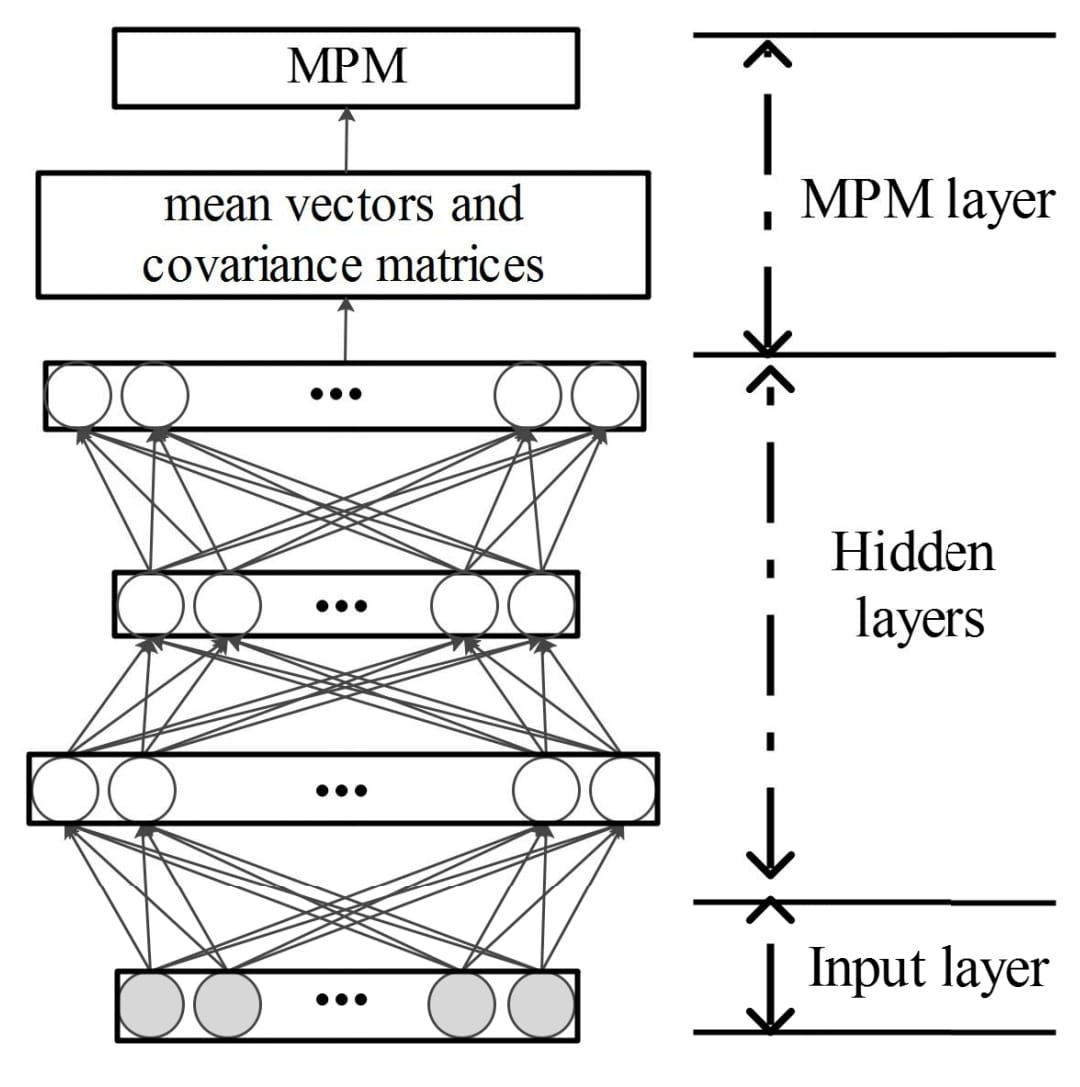
\includegraphics[scale=0.19]{figure_research_paper.jpeg}
    \caption{Deep MPM model}
\end{figure}

\end{frame}
\subsection*{MPM}
\begin{frame}[fragile]
\frametitle{Minimax probability machine}
\begin{enumerate}
    \item Minimax Probability Machine (MPM) tries to minimize the upper bound of the probability of misclassification of future data in a worst-case setting.
    \item No assumptions with respect to the data distribution
    are required in MPM, while those assumptions lack generality
    and are often invalid.
\end{enumerate}
\end{frame}
\begin{frame}[fragile]
\frametitle{Minimax probability machine}
Let x and y denote random vectors with mean vectors and covariance matrices given by x $\sim$ ($\overline{x},\sum_x$) and  y $\sim$ ($\overline{y},\sum_y$) respectively in a binary classification problem, where x, $\overline{x}$, y, $\overline{y}$ $\in \mathbb{R}^n$ and $\sum_x, \sum_y \in \mathbb{R}^{n\times n} $.\\

MPM seeks to determine the hyperplane $a^{\top}z = b$ ($a,z \in \mathbb{R}^n$ and $b \in \mathbb{R}$) which separates the two classes of data with maximal probability. The form of the MPM model is as follows:\\
\begin{align}
    \text{max}_{\alpha,a,b} \text{ $\alpha$} \text{ s.t.}&\text{ inf } \pr{a^{\top} x \geq b } \geq \alpha,  \label{1}\\
    &\text{ inf } \pr{a^{\top}y \leq b } \geq \alpha. \nonumber
\end{align}
Where $\alpha$ denotes the worst case accuracy of the future data.

\end{frame}
\begin{frame}[fragile]
\frametitle{Minimax probability machine(contd.)}
    \begin{lemma}
    Given $a\neq 0$ and b, such that $a^{\top}z \leq b $ and $\beta \in [0,1)$, the condition 
    \begin{align}
        \text{ inf }_{y \sim (\overline{y},\sum_y)} \pr{a^{\top}y \leq b } \geq \beta, \nonumber
    \end{align}
    holds if and only if $b-a^{\top} \overline{y} \geq \kappa(\beta)\sqrt{a^{\top}\sum_y a}$ with $\kappa(\beta)=\sqrt{\frac{\beta}{1-\beta}}$.
    \end{lemma}
    By using the above lemma, \eqref{1} can be written as 
    \begin{align}
        \text{max}_{\alpha,a,b} &\text{ $\alpha$} \text{ s.t.}\nonumber\\
        & -b+a^{\top}\overline{x} \geq \kappa(\alpha)\sqrt{a^{\top}\textstyle \sum_x a}\label{eq2}\\
        & b-a^{\top} \overline{y} \geq \kappa(\alpha)\sqrt{a^{\top}\textstyle \sum_y a}\label{eq3}
    \end{align}
    \end{frame}
\begin{frame}[fragile]
\frametitle{Minimax probability machine(contd.)}
Where $\kappa(\alpha)=\sqrt{\frac{\alpha}{1-\alpha}}$.\\
From \eqref{eq2} and \eqref{eq3}, we get 
\begin{align}
    a^{\top} \overline{y}+\kappa(\alpha)\sqrt{a^{\top}\textstyle \sum_y a} \leq b \leq a^{\top}\overline{x}-\kappa(\alpha)\sqrt{a^{\top}\textstyle \sum_x a} \label{eq4}
\end{align}
On eliminating b from \eqref{eq4}, we get
\begin{align}
    a^{\top}(\overline{x}-\overline{y})\geq \kappa(\alpha)\left( \sqrt{a^{\top}\textstyle \sum_x a}+\sqrt{a^{\top}\textstyle \sum_y a}\right) \label{eq5}
\end{align}
\end{frame}
\begin{frame}[fragile]
\frametitle{Minimax probability machine(contd.)}
Without loss of generality, we can set $a^{\top}(\overline{x}-\overline{y})=1$. Thus \eqref{eq5} changes to:
\begin{align}
    \text{max}_{\alpha,a,b} &\text{ $\alpha$} \text{ s.t.} \nonumber\\
    &1\geq \kappa(\alpha)\left( \sqrt{a^{\top}\textstyle \sum_x a}+\sqrt{a^{\top}\textstyle \sum_y a}\right),\\
    &a^{\top}(\overline{x}-\overline{y})=1\nonumber
    \end{align}
    Since, \kappa($\alpha)=\sqrt{\frac{\alpha}{1-\alpha}}$, it increases monotonically with $\alpha$, so maximising $\alpha$ is equivalent to maximising \kappa($\alpha$), \\
    which implies,
    \begin{align}
        \text{min  }\hspace{.2cm} \sqrt{a^{\top}\textstyle \sum_{x} a}+\sqrt{a^{\top}\textstyle \sum_{y} a} \hspace{.5cm} \text{ s.t. } a^{\top}(\overline{x}-\overline{y})=1 \label{eq7}
    \end{align}
\end{frame}
\begin{frame}[fragile]
\frametitle{Minimax probability machine(contd.)}
Any covariance matrix is a symmetric matrix and positive semi-definite.\\
\begin{block}{}
 If M is a positive semi-definite matrix, then there exists a matrix B such that :
\begin{align}
    M=B^{\top}B
\end{align}
\end{block}

So, 
\begin{align}
    \textstyle \sum_{x} = C^{\top}C
\end{align}
And since covariance matrix is positive semi-definite and symmetric, its root will also be symmetric, so $C^{\top}=C$ and thus $\sum_x^{\frac{1}{2}}=C$.\\


So, \eqref{eq7} can be written as:
\begin{align}
    \text{min  }\hspace{.2cm} \sqrt{a^{\top}C^{\top}C a}+\sqrt{a^{\top}D^{\top}D a} \hspace{.5cm} \text{ s.t. } a^{\top}(\overline{x}-\overline{y})=1
\end{align}
\end{frame}
\begin{frame}[fragile]
\frametitle{Minimax probability machine(contd.)}
\begin{align}
    \text{min  }\hspace{.2cm} \sqrt{(Ca)^{\top}C a}+\sqrt{(Da)^{\top}D a} \hspace{.5cm} \text{ s.t. } a^{\top}(\overline{x}-\overline{y})=1 \label{eq11}
\end{align}
\eqref{eq11} can be written as:
    \begin{align}
    \text{min  }\hspace{.2cm} \norm{(\textstyle \sum_{x})^{\frac{1}{2}} a}+ \norm{(\textstyle \sum_{y})^{\frac{1}{2}} a} \hspace{.5cm} \text{ s.t. } a^{\top}(\overline{x}-\overline{y})=1
\end{align}
 This optimization problem is a second order cone program problem, after obtaining the optimal solution $a_{*},b_{*}$ for a new data point z, if $a_{*}z\geq b_{*}$, z is classified as class x, otherwise z belongs to the class y.
\end{frame}
\subsection*{Deep MPM}
\begin{frame}[fragile]
\frametitle{Deep Minimax probability machine}
\begin{enumerate}
    \item Now we combine the MPM with deep neural networks for the sake of their complementary strengths in the classification task and robustness learning.
    \item MPM can directly minimize the maximum probability
of misclassification with mean vectors and covariance matrices
of the data considering the global structural information.
\end{enumerate}

\end{frame}
\begin{frame}[fragile]
\frametitle{Deep MPM (contd.)}
Let $g(x,w)$ denotes a nonlinear mapping given by a deep
neural network, parametrized by weight $w$. Through a neural network, we obtain effective representation for two classes of data $g(x,w)$ and $g(y,w)$ respectively, making mean vectors and covariance matrices reliable.
\begin{align}
    x \sim (\overline{x},\textstyle \sum_x)\rightarrow  g(x,w) \sim \left(\overline{g(x,w)},\textstyle \sum_{g(x,w)}\right)\\
    y \sim (\overline{y},\textstyle \sum_y)\rightarrow  g(y,w) \sim \left(\overline{g(y,w)},\textstyle \sum_{g(y,w)}\right)
\end{align}
 where $\overline{g(x,w)},\overline{g(y,w)}$ denote mean vectors of two classes of data respectively, and $\sum_{g(x,w)}, \sum_{g(y,w)}$ denote covariance matrices of two classes of data respectively. For simplicity, we omit the parameter w of g(·) in further equations.
\end{frame}
\begin{frame}[fragile]
\frametitle{Deep MPM (contd.)}
We desire a hyperplane $a^{\top}g(z) = b$ that separates the
two classes of data points with maximal probability given the
means and covariance matrices obtaining by a deep neural
network. The formulation of our model is 
\begin{align}
    \text{max}_{\alpha,a,b} \text{ $\alpha$} \text{ s.t.}&\text{ inf } \pr{a^{\top} g(x)\geq b } \geq \alpha,\label{eq1}\\
    &\text{ inf } \pr{a^{\top} g(y) \leq b } \geq \alpha. \nonumber
\end{align}
On simplifying in the similar way that is done in MPM, we get
\begin{align}
    \text{min  }\hspace{.2cm} \sqrt{a^{\top}\textstyle \sum_{g(x)} a}+\sqrt{a^{\top}\textstyle \sum_{g(y)} a} \hspace{.5cm} \text{ s.t. } a^{\top}(\overline{g(x)}-\overline{g(y)})=1
\end{align}
In order to train our model in an end-to-end fashion, we
employ the Lagrangian multiplier method to perform optimization.

\end{frame}
\begin{frame}[fragile]
\frametitle{Deep MPM (contd.)}
With the introduction of a Lagrange multiplier $\lambda$, we can minimize the objective function,
\begin{align}
    \Lagr=\sqrt{a^{\top}\textstyle \sum_{g(x)} a}+\sqrt{a^{\top}\textstyle \sum_{g(y)} a}-\lambda(a^{\top}(\overline{g(x)}-\overline{g(y)})-1)
\end{align}
Now, this is trained with back propagation in an end-to-end fashion, using the chain rule to calculate derivatives about all the parameters.The derivative of weight w is written as:
\begin{align}
    \frac{\partial \Lagr}{\partial w} = &\frac{\partial \Lagr}{\partial \textstyle \sum_{g(x)}}\frac{\partial \textstyle \sum_{g(x)}}{\partial g(x)}\frac{\partial g(x)}{\partial w}+\frac{\partial \Lagr}{\partial \textstyle \sum_{g(y)}}\frac{\partial \textstyle \sum_{g(y)}}{\partial g(y)}\frac{\partial g(y)}{\partial w}+ \nonumber\\
    & + \frac{\partial \Lagr}{\partial \overline{g(x)}}\frac{\partial \overline{g(x)}}{\partial g(x)}\frac{\partial g(x)}{\partial w}+\frac{\partial \Lagr}{\partial \overline{g(y)}}\frac{\partial \overline{g(y)}}{\partial g(y)}\frac{\partial g(y)}{\partial w}
\end{align}
To optimise the model, Nesterov momentum version of mini-batch
SGD is used.

\end{frame}
\begin{frame}[fragile]
\frametitle{Deep MPM (contd.)}
With the optimised parameters $w_{*}, a_{*}$, we obtain $b_{*}$ and $\alpha_{*}$ as,
\begin{align}
    b_{*}=a_{*}^{\top}\overline{g(x)}-\frac{\sqrt{a_{*}^{\top}\textstyle \sum_{g(x)} a_{*}}}{\sqrt{a_{*}^{\top}\textstyle \sum_{g(x)} a_{*}}+\sqrt{a_{*}^{\top}\textstyle \sum_{g(y)} a_{*}}}\\
    \alpha_{*}=\frac{1}{(\sqrt{a_{*}^{\top}\textstyle \sum_{g(x)} a_{*}}+\sqrt{a_{*}^{\top}\textstyle \sum_{g(y)} a_{*}})^2+1}
\end{align}
$\alpha_{*}$ represents worst case accuracy of the future data.In
general, machine learning is fully data-driven, with
the goal of maximizing the accuracy of the known data in the
average sense, while our model is to maximize the accuracy
of the future data in the worst sense, which is more robust.
\end{frame}
\begin{frame}[fragile]
\frametitle{Experiments}
We test our model on MNIST and CIFAR-10 datasets. We train ten binary classifiers with CNN and DeepMPM.
\begin{enumerate}
    \item \textbf{MNIST}: Modified National Institute of Standards and Technology - is a dataset of 60,000 small square 28×28 pixel grayscale images of handwritten single digits between 0 and 9.
    \item \textbf{CIFAR-10}: Canadian Institute For Advanced Research - it contains 60,000 32$\times$32 color images in 10 different classes. The 10 different classes represent airplanes, cars, birds, cats, deer, dogs, frogs, horses, ships, and trucks. There are 6,000 images of each class.
    \item \textbf{CNNs}: CNNs are type of deep neural networks which work best on visual images, using an architecture of sliding filters and convolutional input layers.
    \item \textbf{FGSM attack}: One of the first and most popular adversarial attacks to date is referred to as the Fast Gradient Sign Attack (FGSM).
\end{enumerate}

\end{frame}
\begin{frame}[fragile]
\frametitle{Experiment MNIST}
\begin{figure}
    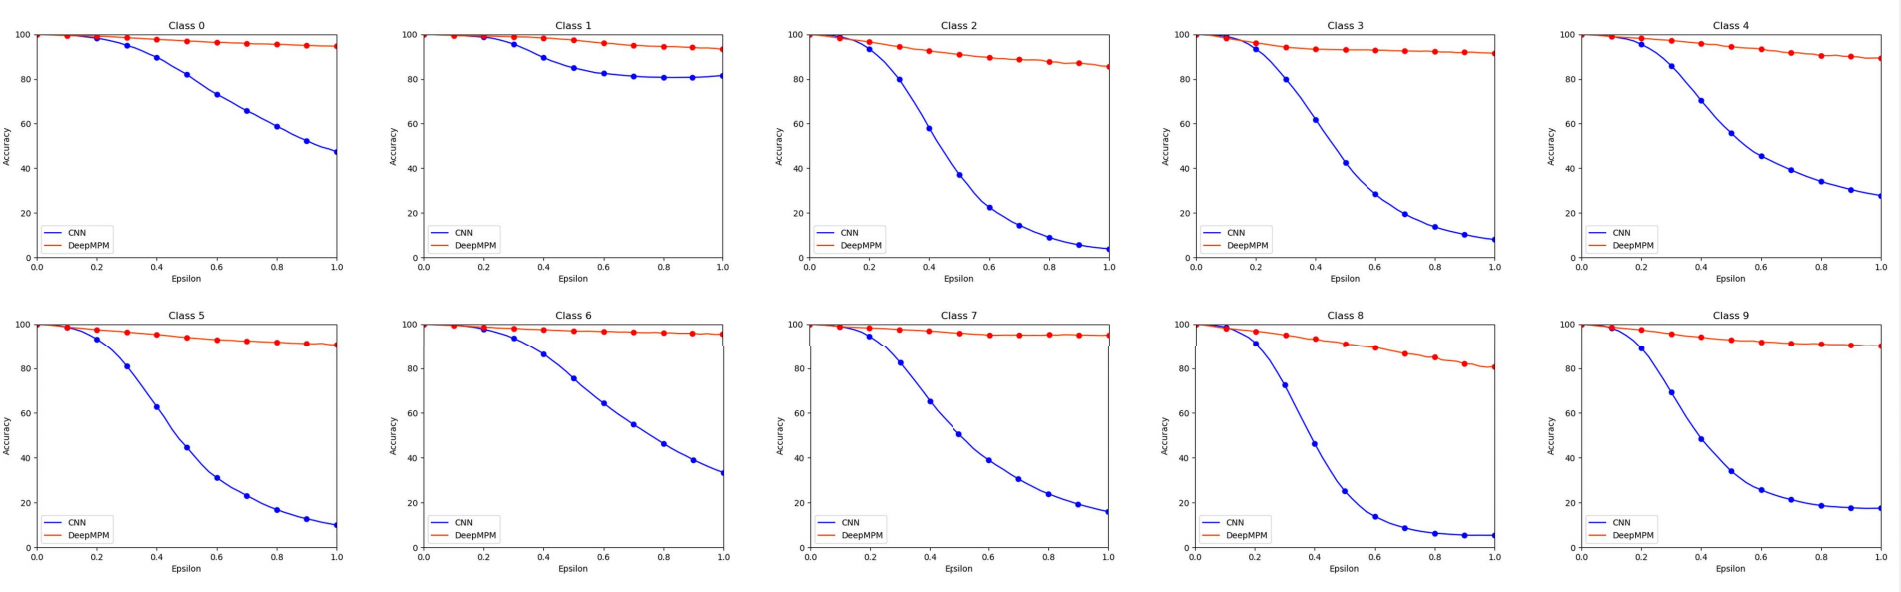
\includegraphics[scale=0.3]{simulations_rp.png}
    \caption{The accuracy of ten binary classifiers on MNIST for FGSM attacks. The horizontal axis represents the size of $\epsilon$. It’s seen that the Accuracy of the DeepMPM decreases much more slowly with the size of adversarial perturbation for all ten classifiers. Thus, DeepMPM is more robust}
\end{figure}
\end{frame}

\begin{frame}[fragile]
\frametitle{Experiment CIFAR-10}
\begin{figure}
    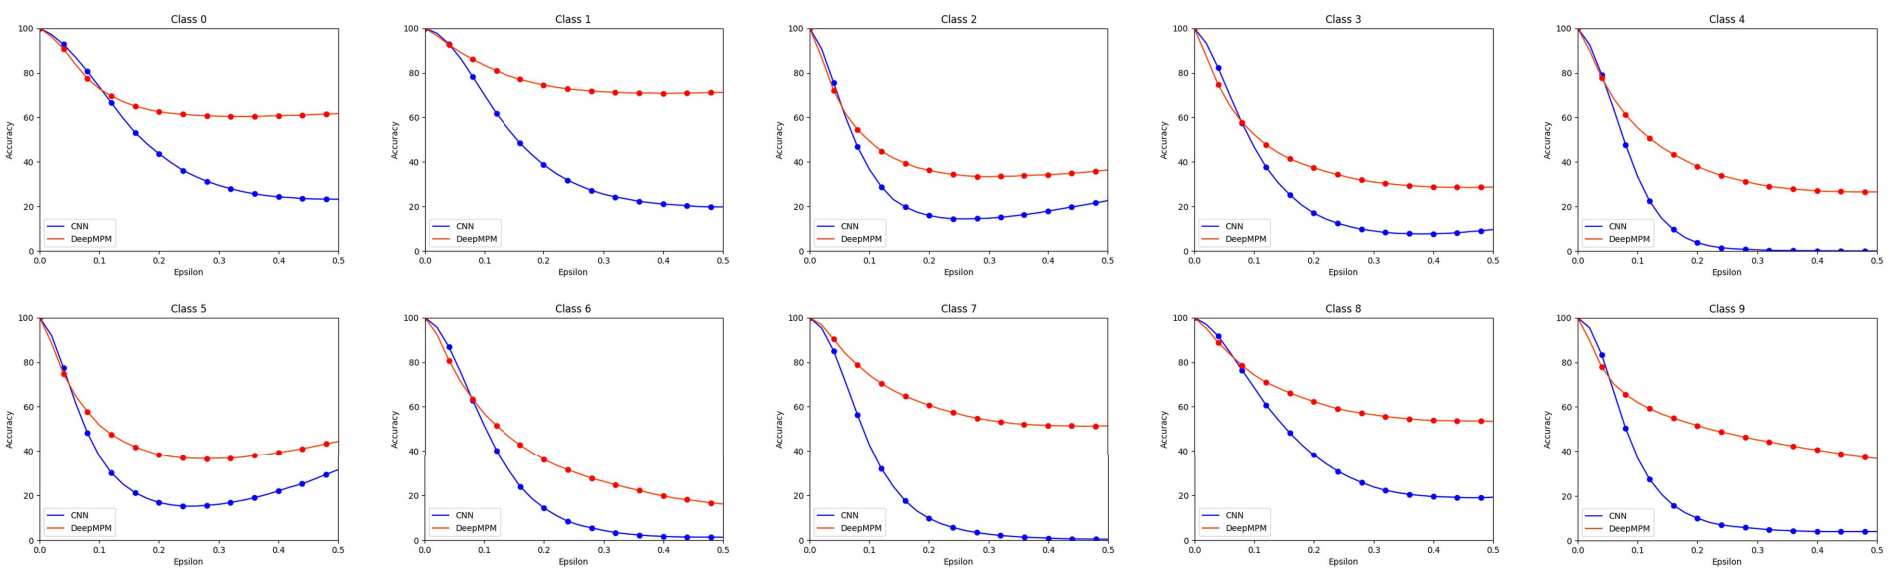
\includegraphics[scale=0.3]{simulation_1_rp.png}
    \caption{The accuracy of ten binary classifiers from the FGSM attacks on CIFAR-10. DeepMPM’s accuracy decreases significantly slower with size of
adversarial perturbation}
\end{figure}
\end{frame}
\end{document}